\newpage
\section{Determinative vs Probabilisitc}
以抠图与去模糊为例.

\subsection{Matting}

\subsubsection{Compositing}
抠图的目的就是合成. 
\begin{itemize}
    \item $F$ 前景
    \item $\alpha$ 透明度
    \item $B$ 背景
    \item $C$ 合成的图像
\end{itemize}
合成公式:
\begin{align*}
    C= \alpha F+(1-\alpha )B
\end{align*}

\subsubsection{Matting}
从 $C$ 分解出 $F, \alpha, B$. 不是唯一解, 病态问题.

Three approaches:
\begin{enumerate}
    \item 减少未知数
    \item 增加观测(约束)
    \item 增加先验(priors)
\end{enumerate}

\paragraph{reduce \# unknowns} difference matting, i.e. known $B$. 用 $C-B$ 得到一个背景的 $\alpha$. 但背景复杂, 所以使用简单的 $B$, 保障 $\alpha$ 的干净. 但纯色的 $B$ 难以获得. 

\paragraph{add observations} 增加不同颜色的 $B$. 

\paragraph{add priors} 若是自然图像, 只能使用这种方法. 
\begin{enumerate}
    \item 用轮廓线算法分割前景与背景, 但轮廓线周围的像素比较 ambiguous. 把图像分成三个区域(trimap), 必定前景/背景, 与轮廓线周围的模糊区域. 
    \item Bayesian framework
\end{enumerate}

\subsubsection{Bayesian framework}
最大化后验概率. 
    
\begin{figure}[!htb]
    \centering
    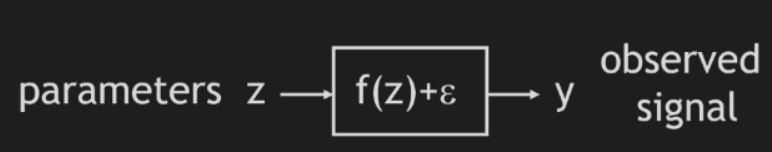
\includegraphics[width=0.42\textwidth]{pic/ACG9/Bayesian framework}
    \caption{Bayesian framework}
\end{figure}
这里 $\epsilon$ 为噪声.

复习下贝叶斯定理: 
\begin{align*}
    P(z|y)P(y)=P(y|z)P(z)
\end{align*}

\begin{align*}
    z^*&=\max_zP(z|y)\\
    &=\max_z\frac{P(y|z)P(z)}{P(y)}\\
    &=\max_z L(y|z)+L(z)
\end{align*}
这里 $L(z)=\log(P(z))$. 因为 $L(y)$ 不影响 $z^*$, 所以舍弃了.

假设 $P(y|z)$ 满足正态分布:
\begin{align*}
    \frac{1}{\sigma\sqrt{2\pi}}e^{-\frac{1}{2}\left( \frac{x-\mu}{\sigma} \right)^2}
\end{align*}

那么
\begin{align*}
    L(y|z)=\frac{\norm{y-f(z)}^2}{\sigma^2}
\end{align*}
表示 data evidence(数据置信度). $L(z)$ 需要使用另一个先验. 

目标问题:
\begin{align*}
    \argmax_{F, B, \alpha}&P(F, B, \alpha|C)\\
    &=\argmax_{F, B, \alpha}\frac{P(C|F, B, \alpha)P(F)P(B)P(\alpha)}{P(C)}\\
    &=\argmax_{F, B, \alpha} L(C|F, B, \alpha)+L(F)+L(B)+L(\alpha)
\end{align*}
这里 $P(C|F, B, \alpha)$ 为 likehood, $P(F)P(B)P(\alpha)$ 为 priors, $P(F, B, \alpha|C)$ 为 posterior proability. 


\begin{figure}[!htb]
    \centering
    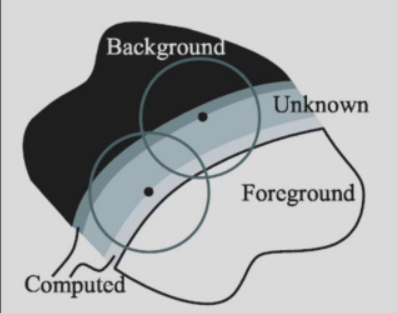
\includegraphics[width=0.309\textwidth]{pic/ACG9/priors.png}
    \caption{$L(F)$ 与 $L(B)$}
\end{figure}

且
\begin{align*}
    L(C|F, B, \alpha)&=-\frac{\norm{C- \alpha F-(1-\alpha)B}^2}{2\sigma_C^2}\\
    L(F)&=-(F-\bar{F})^\top \Sigma_F^{-1}(F-\bar{F})/2\\
    L(B)&=-(B-\bar{B})^\top \Sigma_B^{-1}(B-\bar{B})/2\\
\end{align*}
$\Sigma_F, \Sigma_B$ 为协方差矩阵. 忽略 $L(\alpha)$. 

求解:
\begin{enumerate}
    \item 先固定 $\alpha$ 求解 $F, B$
    \item 再固定 $F, B$ 求解 $\alpha$
\end{enumerate}
迭代直到收敛. 

最后相当于用概率论, 结合已知的先验, 对 $F, B, \alpha$ 进行约束, 让其结果符合先验. 


\subsection{Image Deblurring}

\subsubsection{Different Types of Blur}
三种类型:
\begin{enumerate}
    \item 运动模糊(Scene motion)
    \item 景深(Defocus blur)
    \item 相机抖动(Camera shake)
\end{enumerate}


对于相机抖动, 定义 Convolution 模型. 
\begin{figure}[!htb]
    \centering
    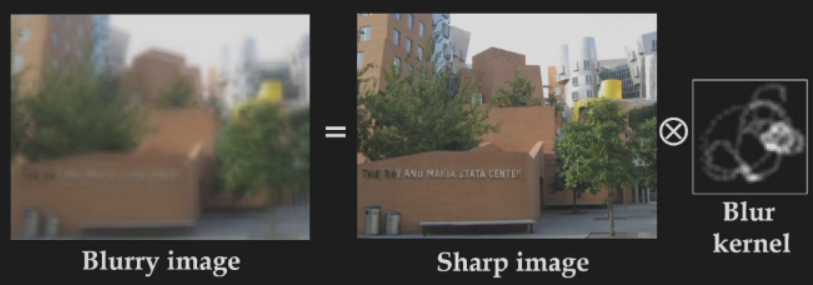
\includegraphics[width=0.42\textwidth]{pic/ACG9//convolution}
    \caption{Convolution}
\end{figure}

目标: 给予 Blurry image, 获得 Sharp image. 假设静态的场景. 

基本上解法分两类: blind v.s. non-blind deconvolution.
\begin{itemize}
    \item non-blind: 已知 blur kernel
    \item blind: 都未知
\end{itemize}

前人的工作有很多的前提假设:
\begin{itemize}
    \item 需要多个图像
    \item 相机运动是简单的
\end{itemize}

即使是 non-blind, 问题仍是病态的. 

\subsubsection{Natural Images Priors}
用梯度分布作为先验, 在自然界中, 图像的梯度是稀疏的. 

\begin{figure}[!htb]
    \centering
    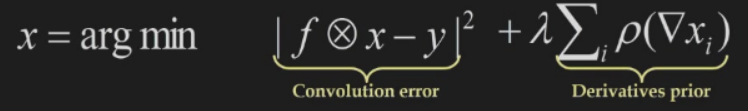
\includegraphics[width=0.42\textwidth]{pic/ACG9/deconvolution with priors}
    \caption{deconvolution with priors}
\end{figure}

然后就是讲论文了
\subsubsection{用一张图消除相机抖动}
需要三种信息:
\begin{enumerate}
    \item 重建约束
    \item 图像先验(图片梯度的分布)
    \item 模糊先验(正+稀疏)
\end{enumerate}

然后就是推公式, 每个值是怎么来的. 摸了!

有问题, 因为先验还是不好, 去模糊后会有噪声. 

\subsubsection{如何做高质量的去模糊}
框架无改变. 引入了图像局部约束, 在模糊图像中, 小梯度的区域, 在清晰图像中, 梯度应该也很小. 

优化的公式涉及卷积, 求解时开销巨大. 使用变量替换的技巧把卷积独立. 还做了个傅里叶变换, 把卷积操作变为乘法操作. 